%Matteo Kumar - Leonard Schatt
% Fortgeschrittenes Physikalisches Praktikum
% Main-Datei für die Auswertung in TeX

% Struktur:
% Für jeden Abschnitt gibt es einen Ordner, damit jeder individuell an seinen Aufgaben arbeiten
% kann, ohne beim merge in GitHub Konflikte zu erhalten. Deshalb werden alle Unteraufgaben auch 
% extra in Ordner angelegt. Die einzelnen Dateien über den input Befehl einfügbar.
% Bilder und andere Grafik werden im Ordner Grafik abgelegt 


% Packages
\documentclass[paper=a4,bibliography=totoc,BCOR=10mm,twoside,numbers=noenddot,fontsize=11pt]{scrreprt}
\usepackage[english]{babel}
\usepackage[latin1, utf8]{inputenc}
\usepackage[babel]{csquotes} %For Quotes
\usepackage[T1]{fontenc}
\usepackage{lmodern}
\usepackage{graphicx}
\usepackage{nicefrac}
\usepackage{fancyvrb}
\usepackage{amsmath,amssymb,amstext}
\usepackage{siunitx}
\usepackage{physics}


%\usepackage{url}  % Wird schon in hyperref importiert
\usepackage{natbib}
\usepackage{microtype}
\usepackage[format=plain]{caption}
\usepackage{titleref}

% Zusätzliche Packages
\usepackage{geometry}
\usepackage{anyfontsize}
\usepackage[table]{xcolor}
\usepackage{ifthen}
\usepackage[absolute,overlay]{textpos}
\usepackage{amsfonts}
\usepackage{xstring}
%\usepackage{tikz}
%\usepackage{pdfpages}
\usepackage{booktabs}
\usepackage{hyperref}
\usepackage[capitalize]{cleveref}
\usepackage{subcaption}



% Abschnittseinrückung und -abstand
% Die folgenden Zeilen sollen möglichst nicht verändert werden
\parindent 0.0cm
\parskip 0.8ex plus 0.5ex minus 0.5ex

% Anzahl und Größe von Gleitobjekten
% maximal 2 Objekte oben und unten
% erlaubt auch größere Bilder, welche die ganze Seite benötigen
% Die folgenden Zeilen sollen möglichst nicht verändert werden
\setcounter{bottomnumber}{2}
\setcounter{topnumber}{2}
\renewcommand{\bottomfraction}{1.}
\renewcommand{\topfraction}{1.}
\renewcommand{\textfraction}{0.}
\AtBeginDocument{\RenewCommandCopy\qty\SI}


%\sc und \bc veraltet. Daher: (20.09.2018)
\DeclareOldFontCommand{\sc}{\normalfont\scshape}{\@nomath\sc}
\DeclareOldFontCommand{\bf}{\normalfont\scshape}{\textbf}

% Verschiedenes
\pagestyle{headings}          % Der Seitenstil sollte möglichst nicht verändert werden
\graphicspath{{./bilder/}}    % Der Pfad für die Abbildungen Abbildungen wird gesetzt
\VerbatimFootnotes            % \verb etc.

% Funktionen
\newcommand\tab[1][1cm]{\hspace*{#1}}
\newcommand{\vect}[1]{\boldsymbol{\mathbf{#1}}}
\newcolumntype{g}{>{\columncolor[rgb]{ .741,  .843,  .933}}l}

%Setup Caption etc.
\captionsetup[figure]{labelfont={bf}}



\begin{document}

    \nonfrenchspacing

    % 0. Kapitel 
    \begin{titlepage}
    \centering
    \vspace*{3cm}
    {\Huge \textbf{Internship AWI} \\[3ex]}
    \vfill
    {\large \textbf{Author}: Leonhard Schatt\\
    \textbf{Supervisor}: Felix Pithan}\\[1ex]
    {\today}


    \newpage
\end{titlepage}

\newpage

\restoregeometry



    \thispagestyle{empty}
    \cleardoublepage
    \tableofcontents
    \cleardoublepage

    % 1. Kapitel Einleitung
    %Matteo Kumar - Leonard Schatt
% Fortgeschrittenes Physikalisches Praktikum

% 1. Kapitel Einleitung

\chapter{Introduction}
\label{chap:einleitung}

In the following, we are going to investigate the effects of nanoplasmonics. As nanostructuring is gaining importance in science and industry, for example in the context of computing or building organic solar cells, this presents a great opportunity to be introduced to this field. Nanoplasmonics is the study of the effects of plasmons, which are strongly confined to the nanoscale. This confinement connects the classical phenomena of plasmons to the world of quantum mechanics. This reappearance of the discretization of energy levels due to the confinement allows the observer to extract information from the sample well below the diffraction limit of $\frac{\lambda}{2}$. 


    % 2.Kapitel Fragen zur Vorbereitung
    %Matteo Kumar - Leonard Schatt
% Fortgeschrittenes Physikalisches Praktikum
 
\chapter{Theory}
\label{cha:theory}




    % 3.Kapitel Protokoll
    %
% Physikalisches Praktikum

% 3.Kapitel  Protokoll

% Variables
\def\skalierung{0.65}

\chapter{Materials, Methods and Setup}
\label{chap:methods}

\section{Dark-field microscopy}
\label{sec:DarkFMicro}

The following section explains the set-up for dark field microscopy and the process of adjustment. 

\subsection{Setup}

The setup itself consist of a system of lenses, a light source one mask and one camera as schematically depicted in \cref{fig:DarkFMicro}. 
In our case all components were realized in a plug system of ThorLabs. We used a white LED as light source and a weak LASER to improve our adjustment of the setup. 
The setup is briefly introduced by following the path of the light. 

\begin{figure}[ht]
    \centering
    \includegraphics[width = \linewidth]{Bilder/Setup/MikroskopEdit.png}
    \caption{Schematic representation of the used dark-field microscope. From \cite{LehrstuhlExperimentalphysikIII.2023}}
    \label{fig:DarkFMicro}
\end{figure}

The first lense parallelizes the light. After this a dark field mask (DF mask) blocks the light which would directly enter in teh second lense of the microscope. The light which is transmitted by the DF mask is guided onto the sample and 
is scattered by the structure. This scattered light is picked up by the lense after the sample and converted to an image using the rest of the lenses. This picture is captured by the camera.

\subsection{Adjusting the setup}

The setup adjustment consists of multiple steps. Firstly, the positioning of the first lens is adjusted. Next, the second lens is focused on the sample, followed by guiding the beam into the spectrometer using two mirrors.

To adjust the position of the first lens, we incorporate a beam splitter in the beam path before the lens. The lens is then focused on the sample. To verify the focus we aim for a sharp image of the reflection, which can be observed through the beam splitter, as shown in Figure \ref{fig:subfig1}.
For this the position of the sample has to be changed using the millimeter screws until we see a the nano particles.


\begin{figure}[ht]
    \centering
    \begin{subfigure}{0.3\linewidth}
      \includegraphics[width=\linewidth]{data/Gruppe2/image_0.png}
      \caption{}
      \label{fig:subfig1}
    \end{subfigure}
    \begin{subfigure}{0.3\linewidth}
      \includegraphics[width=\linewidth]{data/Gruppe2/image_1.png}
      \caption{}
      \label{fig:subfig2}
    \end{subfigure}
    \begin{subfigure}{0.3\linewidth}
      \includegraphics[width=\linewidth]{data/Gruppe2/image_2.png}
      \caption{}
      \label{fig:subfig3}
    \end{subfigure}

    \begin{subfigure}{0.3\linewidth}
      \includegraphics[width=\linewidth]{data/Gruppe2/image_3.png}
      \caption{}
      \label{fig:subfig4}
    \end{subfigure}
    \begin{subfigure}{0.3\linewidth}
      \includegraphics[width=\linewidth]{data/Gruppe2/image_4.png}
      \caption{}
      \label{fig:subfig5}
    \end{subfigure}
    \begin{subfigure}{0.3\linewidth}
      \includegraphics[width=\linewidth]{data/Gruppe2/image_5.png}
      \caption{}
      \label{fig:subfig6}
    \end{subfigure}


    \begin{subfigure}{0.3\linewidth}
      \includegraphics[width=\linewidth]{data/Gruppe2/image_6.png}
      \caption{Horizontal polarizations}
      \label{fig:subfig7}
    \end{subfigure}
    \begin{subfigure}{0.3\linewidth}
      \includegraphics[width=\linewidth]{data/Gruppe2/image_7.png}
      \caption{Vertical polarizations}
      \label{fig:subfig8}
    \end{subfigure}
    \begin{subfigure}{0.3\linewidth}
      \includegraphics[width=\linewidth]{data/Gruppe2/image_8.png}
      \caption{}
      \label{fig:subfig9}
    \end{subfigure}
    
    \caption{The pictures were generated during adjustment of the setup. (a) shows the reflection of the film captured with a camera positioned at the place of the beam splitter. The pictures (b)-(i) ones were taken in transmission, after the adjustment of the second lens.}
    \label{fig:subfigure-grid}
\end{figure}

As a second step, the position of the second lens is optimized using a LASER. The LASER is quickly mounted instead of the LED. The diameter of the LASER spot is minimized by changing the distance of the second lens.

After inserting a second beam splitter following the second lens, we are able to view the transmission picture using a camera, as shown in \cref{fig:subfig2,fig:subfig3,fig:subfig4,fig:subfig5,fig:subfig6,fig:subfig7,fig:subfig8,fig:subfig9}. The contrast increasing effects
of the dark-field microscopy can be easily seen in \cref{fig:subfigure-grid} after placing the DF mask. The positioning of the mask gives artefacts as can be seen in comparing \cref{fig:subfig2,fig:subfig9}. The sample is examined to determine its position by identifying the markers present non its edges. In \cref{fig:subfig7,fig:subfig8,fig:subfig9}, the marker with text can be seen in the bottom left corner. 
By comparing this to the plan for the sample depicted in \cref{fig:NanoDotSketch} and taking into account the orientation of the 
letters on the marker, we can tell that the sample is orientated as on the plan. When inserting polarizations filters as done in \cref{sub@fig:subfig7,sub@fig:subfig9}, we can not notice a difference in the scattering without numerical analysis. A slight shift in color might be visible.  
 

\begin{figure}[ht]
    \centering
    \includegraphics[width = 0.8\linewidth]{Bilder/Setup/SchemeDots.png}
    \caption{Schematic representation of the nano dot structure used. From \cite{LehrstuhlExperimentalphysikIII.2023}}
    \label{fig:NanoDotSketch}
\end{figure}

Afterwards, the beam is directed into the spectrometer by utilizing two mirrors. The slit is fully opened. Using the spectrometer, we examine a small image captured through the slit, which allows us to determine our location on the sample by identifying distinctive contaminants present. Once the sample position is determined, we reduce noise by closing the slit and manually positioning the sample using the second beam splitter and the camera to orient ourselves on the sample. When it comes to measurement, we remove both beam splitters.
\section{Sample}
\label{sec:sample}

The sample used is a sample of nanorods depicted in \ref{fig:NanoDotSketch}. 
The sample was created through electron beam lithography. It is placed on a cover glass (BK7) with an estimated thickness of around \SI{170}{\micro\meter}. The structure stands at a height of \SI{35}{\nano\meter} and is composed of silver, where in contrast to gold, all electrons can be approximated as free electrons. Due to the writing and deposition process, the structure is planar and consists of nanorods with widths of \SI{70}{\nano\meter} and \SI{90}{\nano\meter} and variable length L. The length of the nanorods, denoted as L, is varied.

    % 4.Kapitel Versuchsauswertung
    % Matteo Kumar - Leonard Schatt
% Fortgeschrittenes Physikalisches Praktikum
% 4.Kapitel Versuchsauswertung

\chapter{Discussion of the Ensemble Measurement}
\label{chap:versuchsauswertung}

% Matteo Kumar - Leonard Schatt
% Fortgeschrittenes Physikalisches Praktikum
% 4.Kapitel Versuchsauswertung


For the ensemble measurements the fourteen samples of rods of different lengths and widths were measured with unpolarized light and light of \ang{0} and \ang{90} polarization each. The measured spectra $I_m$ were corrected using a reference spectrum $I_r$ taken without a sample for each of the three polarization setups. The corrected spectra $I_c$ were thus calculated as
\begin{equation}
    I_c = \frac{I_m}{I_r}.
\end{equation}
Although a dark spectrum $I_d$ was taken as well, it was not used for this evaluation, since $I_m$, $I_r$ and $I_d$ converged to the same intensities for increasing wavelengths and therefore created singularities when subtracting $I_d$ from both $I_m$ and $I_r$. This could be done since the values for $I_d$ were constant and small for the relevant parts of the wavelength scale. The corrected spectra can be seen in fig.~\ref{fig:unpol}, \ref{fig:pol0} and \ref{fig:pol90}. Using a gaussian function the wavelength for the maximum intensity $\lambda_{max}$ was calculated. All values can be found in tab.~\ref{tab:lamMaxUn},~\ref{tab:lamMax0} and \ref{tab:lamMax90}.

\begin{figure}
    \centering
    \begin{subfigure}{\textwidth}
        \includegraphics[width=\textwidth]{Bilder/Auswertung/SpektrumUnpol70.png}
        \caption{ }
        \label{fig:u70}
    \end{subfigure}
    \hfill
    \begin{subfigure}{\textwidth}
        \includegraphics[width=\textwidth]{Bilder/Auswertung/SpektrumUnpol90.png}
        \caption{ }
        \label{fig:u90}
    \end{subfigure}
    \caption{The corrected spectra of the samples using unpolarized light are shown. While the rodlength varied throughput the samples, the rodwith of \SI{70}{\nano\meter} was fixed in (a) and one of \SI{90}{\nano\meter} in (b).}
    \label{fig:unpol}
\end{figure}

\begin{figure}
    \centering
    \begin{subfigure}{\textwidth}
        \includegraphics[width=\textwidth]{Bilder/Auswertung/SpektrumPol070.png}
        \caption{ }
        \label{fig:0-70}
    \end{subfigure}
    \hfill
    \begin{subfigure}{\textwidth}
        \includegraphics[width=\textwidth]{Bilder/Auswertung/SpektrumPol090.png}
        \caption{ }
        \label{fig:0-90}
    \end{subfigure}
    \caption{The corrected spectra of the samples using polarized light of \ang{0} are shown. While the rodlength varied throughput the samples, the rodwith of \SI{70}{\nano\meter} was fixed in (a) and one of \SI{90}{\nano\meter} in (b).}
    \label{fig:pol0}
\end{figure}

\begin{figure}
    \centering
    \begin{subfigure}{\textwidth}
        \includegraphics[width=\textwidth]{Bilder/Auswertung/SpektrumPol9070.png}
        \caption{ }
        \label{fig:90-70}
    \end{subfigure}
    \hfill
    \begin{subfigure}{\textwidth}
        \includegraphics[width=\textwidth]{Bilder/Auswertung/SpektrumPol9090.png}
        \caption{ }
        \label{fig:90-90}
    \end{subfigure}
    \caption{The corrected spectra of the samples using polarized light of \ang{90} are shown. While the rodlength varied throughput the samples, the rodwith of \SI{70}{\nano\meter} was fixed in (a) and one of \SI{90}{\nano\meter} in (b).}
    \label{fig:pol90}
\end{figure}

\begin{table}
    \centering
    \begin{tabular}{c|cc}
        \toprule
        $l$ / \si{\nano\meter} &   $\lambda_{max,unpol,w=\SI{70}{\nano\meter}}$ / \si{\nano\meter}& $\lambda_{max,unpol,w=\SI{90}{\nano\meter}}$ / \si{\nano\meter}\\
        \midrule
        70  &  $708.2 \pm 0.4$&  $602.2 \pm 2.8$\\
        80  &  $741.5 \pm 1.0$&  $653.8 \pm 0.4$\\
        90  &  $669.6 \pm 0.3$&  $687.98 \pm 0.08$\\
        100 &  $696.44 \pm 0.18$&  $703.84 \pm 0.10$\\
        110 &  $712.5 \pm 0.3$&  $719.30 \pm 0.16$\\
        120 &  $757.6 \pm 1.4$&  $743.9 \pm 0.4$\\
        130 &  $668.5 \pm 0.4$&  $707.67 \pm 0.15$\\
        140 &  $664.8 \pm 0.3$&  $690.03 \pm 0.12$\\
        \bottomrule
    \end{tabular}
    \caption{Values of the wavelength of the maximum intensity of the spectra in fig.~\ref{fig:unpol}. All values were calculated from a fit using a gaussian function. The error represents the fitting error.}
    \label{tab:lamMaxUn}
\end{table}

\begin{table}
    \centering
    \begin{tabular}{c|cc}
        \toprule
        $l$ / \si{\nano\meter} &   $\lambda_{max,\ang{0},w=\SI{70}{\nano\meter}}$ / \si{\nano\meter}& $\lambda_{max,\ang{0},w=\SI{90}{\nano\meter}}$ / \si{\nano\meter}\\
        \midrule
        70 &  $715.1 \pm 0.3$&  $619.92\pm 0.15$\\
        80 &  $752.4 \pm 0.9$&  $642.88\pm 0.11$\\
        90  &  $688.1\pm 0.3$&  $683.02\pm 0.05$\\
        100 &  $700.21\pm 0.16$&  $699.07\pm 0.09$\\
        110 &  $716.48\pm 0.19$&  $716.39\pm 0.12$\\
        120 &  $751.4\pm 0.6$&  $736.7\pm 0.2$\\
        130 &  $709.5\pm 0.4$&  $715.3\pm 0.2$\\
        140 &  $705.8\pm 0.2$&  $699.33\pm 0.17$\\
        \bottomrule
    \end{tabular}
    \caption{Values of the wavelength of the maximum intensity of the spectra in fig.~ \ref{fig:pol0}. All values were calculated from a fit using a gaussian function. The error represents the fitting error.}
    \label{tab:lamMax0}
\end{table}

\begin{table}
    \centering
    \begin{tabular}{c|cc}
        \toprule
        $l$ / \si{\nano\meter} & $\lambda_{max,\ang{90},w=\SI{70}{\nano\meter}}$ / \si{\nano\meter}& $\lambda_{max,\ang{90},w=\SI{90}{\nano\meter}}$ / \si{\nano\meter}\\
        \midrule
        70  &  $664.06\pm 0.11$&  $687.18\pm 0.4$\\
        80  &  $659.13\pm 0.12$&  $678.41\pm 0.17$\\
        90  &  $651.89\pm 0.08$&  $684.50\pm 07$\\
        100 &  $668.10\pm 0.08$&  $690.46\pm 0.13$\\
        110 &  $668.06\pm 0.11$&  $691.38\pm 0.11$\\
        120 &  $660.99\pm 0.13$&  $688.20\pm 0.10$\\
        130 &  $653.20\pm 0.07$&   $668.06\pm 0.11$\\
        140 &  $649.43\pm 0.06$&  $664.28\pm 0.09$\\
        \bottomrule
    \end{tabular}
    \caption{Values of the wavelength of the maximum intensity of the spectra in fig.~\ref{fig:pol90}. All values were calculated from a fit using a gaussian function. The error represents the fitting error.}
    \label{tab:lamMax90}
\end{table}


    
As well in fig.~\ref{fig:pol90} as in tab.~\ref{tab:lamMax90} can be seen that in the case of a polarization of \ang{90} the wavelength at the maximum of the intensity spectra does not shift with a varying rodlength. This corresponds to the literature which lets us expect no shifting of the maxima for the transversal modes~\cite{LehrstuhlExperimentalphysikIII.2023}. On the other hand, for the longitudinal modes (i.e.~a polarization of \ang{0}), a shift of the maximum can be observed in fig.~\ref{fig:pol0} and in tab.~\ref{tab:lamMax0}, both. The unpolarized spectra should show characteristica of transversal and longitudinal modes, as both are excited. This is the case here, as can be seen especially for $w$ = \SI{90}{\nano\meter} (and e.g.~$l$ = \SI{80}{\nano\meter}). Hereby can be seen, that the peaks for the transversal modes are smaller as the ones of the longitudinal modes (except the cases for $l<w$ for obvious reasons). Further, the calculated maxima for \ang{0} polarization match the calculated maxima for the measurements using unpolarized light. This is a further confirmation of our measurement since \ang{0} polarized light should be part of unpolarized light. \par 
As stated above, the maximum wavelength $\lambda_{max}$ depends on the rodlength when using \ang{0} polarized light. We expect to find a linear correlation, as the literature states 
\begin{equation}
    m \lambda = 2n_{eff}(L(m)+\Delta L),
\end{equation}
with the effective refractive index of the plasmon $n_{eff}$ and its resonator length $L(m)+\Delta L$~\cite{LehrstuhlExperimentalphysikIII.2023}. Using the ground mode ($m=1$) one gets 
\begin{equation}
    \lambda (L) = 2n_{eff}L + 2n_{eff}\Delta L.
\end{equation}
Therefore, a fit was made based on a linear function. This is illustrated in fig.~\ref{fig:rodlength}. Hereby, for $w =$ \SI{70}{\nano\meter} and $w =$ \SI{90}{\nano\meter} the datapoints of $l =$ \SI{130}{\nano\meter} and $l =$ \SI{140}{\nano\meter} as well as the points of $l =$ \SI{70}{\nano\meter} and $l =$ \SI{80}{\nano\meter} just in the case for $w =$ \SI{70}{\nano\meter} were omitted, as they were far off the expectations. In the cases of the former, the intensity curves were very broad (see fig.~\ref{fig:0-70} and~\ref{fig:0-90}) and therefore the maxima may not be calculated as precise as needed.

\begin{figure}
    \centering
    \includegraphics[width=\textwidth]{Bilder/Auswertung/fitRods.png}
    \caption{The maximum wavelength depends linear on the rodlength as the fitted lines show.}
    \label{fig:rodlength}
\end{figure}

Both fitted lines show similar properties. This is up to our expectations since $n_{eff}$ and $\Delta L$ should not depend on the rodlength. Evaluating the slope and y-axis intersection and then averaging over both measurements one yields \par 

\centerline{\boxed{n_{eff} = \num{1.2 \pm 0.3} \qquad \Delta L = \SI{190 \pm 28}{\nano\meter}.}}

$n_{eff}$ seems resonable since a value of $n_{eff} =$1.4 can be used to describe a particle at a water/air interface~\cite{LehrstuhlExperimentalphysikIII.2023}. The values for $\Delta L$ are quite high comparing them with the actual lengths of the rods. That means that the length of the resonator can be over trice the length of the rods themself in our measurements. However, this aligns with the literature, which states, that the plasmonic electrical field outside the plasmon does not exceed \SI{100}{\nano\meter} which would correspond to $\frac{\Delta L}{2}$~\cite{Chen.2013}.

    % 5.Kapitel Fazit
    %Matteo Kumar - Leonard Schatt
% Fortgeschrittenes Physikalisches Praktikum

% 5. Kapitel Einleitung

\chapter{Summary}
\label{chap:sumamry}
In this practical course we had some first insight in the field of plasmonics. With the dark field microscopy we learned a new technique which allows a background free investigation of plasmonics below its actual resolution limit. Therefore, we were able to measure transversal and longitudinal plasmonic modes. Here we could show, that indeed only the longitudinal modes show a maximum wavelength dependence in respect to the rodlength. 



    % Matteo Kumar - Leonard Schatt
% Physikalisches Praktikum

% Anhang

\appendix

% Text

\chapter{Append}
\label{AppChap:Robustness}

\section{Robustness}

\begin{figure}[ht]
    \centering
    \begin{subfigure}{0.48\textwidth}
        \centering
        \includegraphics[width = \textwidth]{C:/Users/leonh/Desktop/Praktikum_AWI/NordPolLinks/Lon_66_70/TMin/TMin_Month_9.png}
        \caption{$T_{min}$ for the left hemisphere between 66 and 70°}
    \end{subfigure}
    \begin{subfigure}{0.48\textwidth}
        \centering
        \includegraphics[width = \textwidth]{C:/Users/leonh/Desktop/Praktikum_AWI/NordPolRechts/Lon_66_70/TMin/TMin_Month_9.png}
        \caption{$T_{min}$ for the right hemisphere between 66 and 70°}
    \end{subfigure}
    
    \begin{subfigure}{0.48\textwidth}
        \centering
        \includegraphics[width = \textwidth]{C:/Users/leonh/Desktop/Praktikum_AWI/NordPolLinks/Lon_70_75/TMin/TMin_Month_9.png}
        \caption{$T_{min}$ between 70 and 75°}
    \end{subfigure}
    \begin{subfigure}{0.48\textwidth}
        \centering
        \includegraphics[width = \textwidth]{C:/Users/leonh/Desktop/Praktikum_AWI/NordPolRechts/Lon_70_75/TMin/TMin_Month_9.png}
        \caption{$T_{min}$ between 70 and 75°}
    \end{subfigure}

        
    \begin{subfigure}{0.48\textwidth}
        \centering
        \includegraphics[width = \textwidth]{C:/Users/leonh/Desktop/Praktikum_AWI/NordPolLinks/Lon_75_80/TMin/TMin_Month_9.png}
        \caption{$T_{min}$ between 75 and 80°}
    \end{subfigure}
    \begin{subfigure}{0.48\textwidth}
        \centering
        \includegraphics[width = \textwidth]{C:/Users/leonh/Desktop/Praktikum_AWI/NordPolRechts/Lon_75_80/TMin/TMin_Month_9.png}
        \caption{$T_{min}$ between 75 and 80°}
    \end{subfigure}

    \begin{subfigure}{0.48\textwidth}
        \centering
        \includegraphics[width = \textwidth]{C:/Users/leonh/Desktop/Praktikum_AWI/NordPolLinks/Lon_80_82/TMin/TMin_Month_9.png}
        \caption{$T_{min}$ between 80 and 82°}
    \end{subfigure}
    \begin{subfigure}{0.48\textwidth}
        \centering
        \includegraphics[width = \textwidth]{C:/Users/leonh/Desktop/Praktikum_AWI/NordPolRechts/Lon_80_82/TMin/TMin_Month_9.png}
        \caption{$T_{min}$ between 80 and 82°}
    \end{subfigure}
    % Include your other subfigures here...
    \caption{Temperature for left and right hemisphere}
    \label{app:MinTemp}
\end{figure}

\begin{figure}[ht]
    \centering
    \begin{subfigure}{0.48\textwidth}
        \centering
        \includegraphics[width = \textwidth]{C:/Users/leonh/Desktop/Praktikum_AWI/NordPolLinks/Lon_66_70/TMax/TMax_Month_9.png}
        \caption{$T_{max}$ for the left hemisphere between 66 and 70°}
    \end{subfigure}
    \begin{subfigure}{0.48\textwidth}
        \centering
        \includegraphics[width = \textwidth]{C:/Users/leonh/Desktop/Praktikum_AWI/NordPolRechts/Lon_66_70/TMax/TMax_Month_9.png}
        \caption{$T_{max}$ for the right hemisphere between 66 and 70°}
    \end{subfigure}
    
    \begin{subfigure}{0.48\textwidth}
        \centering
        \includegraphics[width = \textwidth]{C:/Users/leonh/Desktop/Praktikum_AWI/NordPolLinks/Lon_70_75/TMax/TMax_Month_9.png}
        \caption{$T_{max}$ between 70 and 75°}
    \end{subfigure}
    \begin{subfigure}{0.48\textwidth}
        \centering
        \includegraphics[width = \textwidth]{C:/Users/leonh/Desktop/Praktikum_AWI/NordPolRechts/Lon_70_75/TMax/TMax_Month_9.png}
        \caption{$T_{max}$ between 70 and 75°}
    \end{subfigure}

        
    \begin{subfigure}{0.48\textwidth}
        \centering
        \includegraphics[width = \textwidth]{C:/Users/leonh/Desktop/Praktikum_AWI/NordPolLinks/Lon_75_80/TMax/TMax_Month_9.png}
        \caption{$T_{max}$ between 75 and 80°}
    \end{subfigure}
    \begin{subfigure}{0.48\textwidth}
        \centering
        \includegraphics[width = \textwidth]{C:/Users/leonh/Desktop/Praktikum_AWI/NordPolRechts/Lon_75_80/TMax/TMax_Month_9.png}
        \caption{$T_{max}$ between 75 and 80°}
    \end{subfigure}

    \begin{subfigure}{0.48\textwidth}
        \centering
        \includegraphics[width = \textwidth]{C:/Users/leonh/Desktop/Praktikum_AWI/NordPolLinks/Lon_80_82/TMax/TMax_Month_9.png}
        \caption{$T_{max}$ between 80 and 82°}
    \end{subfigure}
    \begin{subfigure}{0.48\textwidth}
        \centering
        \includegraphics[width = \textwidth]{C:/Users/leonh/Desktop/Praktikum_AWI/NordPolRechts/Lon_80_82/TMax/TMax_Month_9.png}
        \caption{$T_{max}$ between 80 and 82°}
    \end{subfigure}
    % Include your other subfigures here...
    \caption{Temperature for left and right hemisphere}
    \label{app:MaxTemp}
\end{figure}





    % Literatur
    \bibliographystyle{plain}
    \nocite{*}
    \bibliography{Auswertung.bib}

\end{document}